\documentclass{article}

%Librerías
\usepackage[utf8]{inputenc}
\usepackage[spanish,mexico]{babel}
\usepackage{apacite}
\usepackage{pgfgantt}
\usepackage{pgfcalendar}
\usepackage{xcolor}
\usetikzlibrary{shapes}
\definecolor{colorGrupo}{RGB}{36, 85, 112}  % Color rojo (cambia los valores RGB según tus preferencias)
\definecolor{colorSubGrupo}{RGB}{109, 141, 159}


\bibliographystyle{apacite}
%\bibliographystyle{abbrvnat}
\setlength{\textwidth}{18cm}
\setlength{\oddsidemargin}{-1cm}
\setlength{\headsep}{-1cm}
\setlength{\voffset}{0cm}
\setlength{\topmargin}{0cm}
\setlength{\headheight}{0cm}

\usepackage{tikz}
\usepackage{multicol}
\usepackage{lipsum} 
%\bibliographystyle{apacite}
\usepackage[spanish]{babel}
\selectlanguage{spanish}


\begin{document}

%%%%%% ENCABEZADO %%%%%%%%%%%%%%%%%%%%%%%%%%%%%%%%%%%%%%%
% Logo de la maestría
\colorbox{white!10!}{
    \begin{minipage}[t]{0.05\textwidth} %0.165 
       \begin{flushright}
        
\includegraphics[width=2in]{logo UPS.png}
       \end{flushright}
    \end{minipage}
    \begin{minipage}[H]{0.62 \textwidth} %0.62
        \begin{center}
         
        \end{center}
     \end{minipage}
    \begin{minipage}[t]{0.05 \textwidth}
        \begin{flushleft}
        \hspace{10.25cm}
            
\includegraphics[width=2in]{Posgrados.png}
        \end{flushleft}
    \end{minipage}
}

\begin{tikzpicture}
    \draw[thick] (-6.5,0)--(11.2,0);
\end{tikzpicture}
%%%%%%%%%%%%%%%%%%%%%%%%%%%%%%%%%%%%%%%%%%%%%%%%%%%%%%%%%
\vspace{0.1cm}
\begin{center}
{\large\textsc{ANTEPROYECTO DEL TRABAJO DE TITULACIÓN}} \\
\vspace{0.5cm}
{ \large \textbf{Bryam Fernando Cabrera}} \\ 
\vspace{0.25cm}
{ \large \textbf{Willian Ariolfo  Lituma}}
\end{center}
\vspace{0.1cm}

\section{Tema del Trabajo de Titulación:  }
\begin{center}
    Análisis, desarrollo y migración de los módulos de proveedores y clientes del sistema contable de la empresa Accescont para agilizar los procesos relacionados al manejo de la facturación para el departamento financiero de la empresa.
\end{center}
\section{Docente tutor propuesto:   }
\begin{center}
Ing. María Del Pilar Morquecho Yunga, Msc
\end{center}
\section{Antecedentes}

En el dinámico entorno empresarial actual, la gestión eficiente de la tecnología de la información y los sistemas contables se ha convertido en un factor crítico para el éxito de las organizaciones. Accescont, una respetada firma de auditoría financiera con más de 35 años de experiencia con sede en Cuenca, Ecuador, enfrenta desafíos sustanciales derivados de las limitaciones y obsolescencia de su sistema contable actual \cite{CatacoraSI}.

El núcleo de esta problemática radica en la arquitectura monolítica del sistema actual, que ha sido sometido a múltiples modificaciones para adaptarse a las cambiantes necesidades empresariales \cite{HallSIC}. Lamentablemente, estas adaptaciones han desencadenado una degradación significativa del código, comprometiendo la escalabilidad y flexibilidad del sistema. Esta situación presenta una clara amenaza para la capacidad de Accescont de responder ágilmente a nuevas demandas del mercado y de sus clientes.\cite{HorngrenCC}.

Es importante destacar que el éxito de este proyecto de titulación dependerá en gran medida de la colaboración efectiva con los usuarios y las partes interesadas de Accescont. También se hará hincapié en el cumplimiento de los plazos y la ejecución eficiente de las fases planificadas para garantizar el desarrollo efectivo de los módulos antes mencionados.





 %\lipsum[1-1]
       
 \section{Justificación:}

 En el contexto empresarial actual, la tecnología de la información y los sistemas contables desempeñan un papel crítico para el éxito y la eficiencia de las organizaciones. Accescont, una firma de auditoría financiera con más de 35 años de experiencia con sede en Cuenca, Ecuador, se enfrenta a desafíos significativos debido a las limitaciones y la obsolescencia de su sistema contable actual. Este sistema, que ha sido parte integral de la empresa durante años, ha quedado rezagado en términos de funcionalidad y seguridad, lo que dificulta su capacidad para adaptarse a las cambiantes necesidades empresariales y la incorporación de nuevos módulos contables, en especial los módulos de manejo de clientes y proveedores.
 
 El principal problema radica en la arquitectura monolítica del sistema actual, que ha experimentado modificaciones a lo largo del tiempo para satisfacer las necesidades cambiantes de la empresa. Sin embargo, estas modificaciones han llevado a una degradación significativa del código, lo que podría comprometer aún más el sistema en caso de necesitar más cambios. Como resultado, la empresa reconoce la necesidad urgente de implementar un nuevo sistema contable sin afectar a sus clientes existentes.
 
 En base a esta problemática, este proyecto se enmarca en la búsqueda de una solución integral y efectiva para fortalecer las operaciones contables de Accescont, enfocándose en los dos módulos clientes y proceedores considerados los mas criticos para la emrpesa. Estos módulos buscarán superar los desafíos tecnológicos actuales mediante la implementación de nuevas herramientas, como los microservicios, que optimizarán la gestión financiera y contribuirán al crecimiento sostenible de la empresa. Además, este enfoque permitirá el escalamiento y adaptación del sistema con la agregación de otros módulos.
  
 En resumen, este trabajo de titulación busca abordar una problemática real en el ámbito empresarial. Accescont se enfrenta a desafíos tecnológicos y de usabilidad con su sistema contable actual, y el proyecto propuesto tiene como objetivo superar estos desafíos mediante la implementación de una solución innovadora y escalable. La colaboración con los stakeholders y el cumplimiento de los plazos son elementos clave para el éxito de este proyecto y su contribución al crecimiento y competitividad de Accescont en el mercado.
 

\section{Objetivos:}

\subsection{Objetivo General}

Analizar, desarrollar y migrar los módulos de clientes y proveedores del sistema contable de la empresa Accescont en la ciudad de Cuenca.  
\subsection{Objetivos Específicos}

\begin{enumerate}
    \item Analizar los requerimientos para los módulos del nuevo sistema contable con la participación de los usuarios y partes interesadas.
    
    \item Diseñar la arquitectura del sistema contable según los requerimientos establecidos.   
    \item Desarrollar los módulos de clientes y proveedores para el sistema contable que cumpla con los requisitos identificados, usando metodologías ágiles de desarrollo de software con el propósito de que los módulos sean adaptables y escalables para un posterior crecimiento del sistema contable.  
    
    \item Evaluar el desarrollo de los módulos para garantizar su calidad y funcionalidad realizando pruebas de validación y usabilidad, que aseguren un adecuado funcionamiento acorde a los objetivos y requisitos planteados.  
\end{enumerate}


\section{Alcance:}
El proyecto se enfocará en analizar, desarrollar y migrar los módulos de clientes y proveedores dentro del sistema contable de Accescont. Luego de realizar las pruebas minuciozas estos módulos servirán de base para agregar otros nuevos al sistema en al largo plazo.

Es importante resaltar que este proyecto considerará los módulos mas sensibles del sistema contable siendo estos clientes y proveedores debido al impacto que respresentan en las operaciones de la empresa.

Se identificarán los requerimientos de usuario con el objetivo de diseñar los módulos de forma que satisfagan las necesidades de Accescont. Posteriormente se construirán los módulos, incluyendo su programación y configuración, previos a la implementación, para así optimizar la gestión de clientes y proveedores.

Los datos existentes se migrarán de forma controlada a los nuevos módulos, garantizando que no haya pérdida ni errores en la información. Para esto se realizarán pruebas exhaustivas para validar su correcto funcionamiento.

Este proyecto se centra en el desarrollo de los módulos de clientes y proveedores que a largo plazo sentaran las bases para el desarrollo de nuevos módulos que se integraran al sistema contable de Accescont.

\section{Metodología}

Con la finalidad de cumplir con los objetivos específicos planteados en el presente documento, se ha decidido implementar metodologías agiles, lo cual permite dividir el proyecto en pequeñas fases, con objetivos bien definidos y así lograr el desarrollo correcto de los módulos desarrollados.  

\begin{figure}[h]
    \centering
    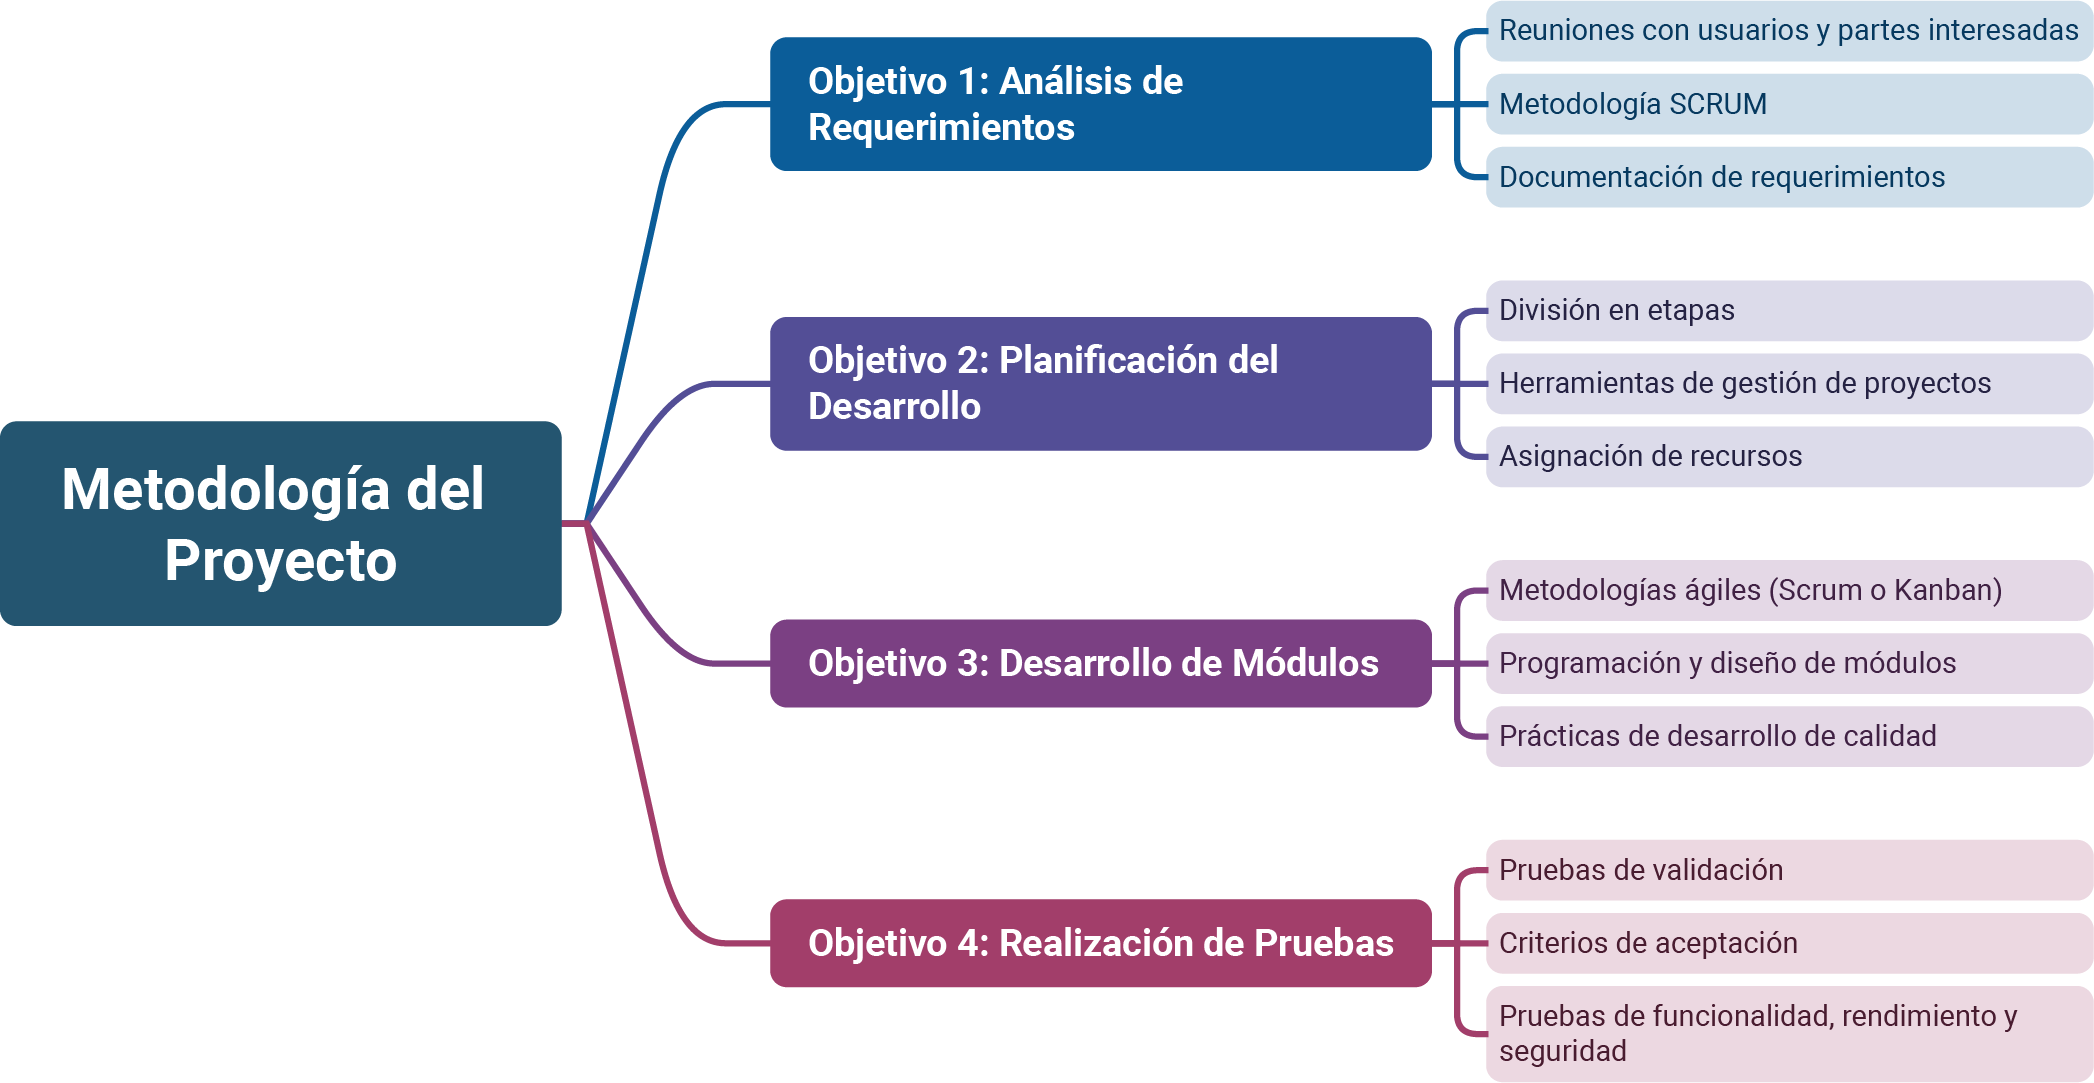
\includegraphics[width=0.8\textwidth]{med.png}
    \caption{Diagrama de flujo del análisis de requerimientos.}
\end{figure}

\subsection{Objetivo 1: Análisis de requerimientos}

Seguira la siguiente metodología

\begin{itemize}
    \item Se llevarán a cabo reuniones con los usuarios y partes interesadas de Accescont para recopilar información detallada sobre los requerimientos.
    \item Se utilizará la metodología SCRUM para facilitar la comunicación con los stakeholders y garantizar una comprensión clara de sus necesidades.
    \item Se documentarán los requerimientos identificados en un documento formal que servirá como base para el desarrollo.
\end{itemize}

\subsection{Objetivo 2: Diseñar la arquitectura del sistema contable}

Seguira la siguiente metodología

\begin{itemize}
    \item Definición precisa de las características y funcionalidades necesarias, incluyendo aspectos de escalabilidad, seguridad, interfaz de usuario e integraciones ente módulos, para asegurar un diseño alineado con las necesidades de Accescont.
    \item Desarrollo de un diseño arquitectónico sólido que visualice la estructura del sistema contable, utilizando herramientas como diagramas de flujo, diagramas de clase, y otros modelos arquitectónicos.
    \item Elaboración de documentos detallados que describan la arquitectura del sistema contable, sus componentes, relaciones y flujos de datos, facilitando la comprensión para los desarrolladores y otros equipos involucrados.
\end{itemize}

\subsection{Objetivo 3: Desarrollo de módulos}

Seguira la siguiente metodología

\begin{itemize}
    \item Se utilizarán metodologías ágiles de desarrollo de software, como Scrum o Kanban, para garantizar la flexibilidad y adaptabilidad durante el proceso de desarrollo.
    \item Se diseñarán y programarán los módulos teniendo en cuenta los requerimientos identificados en el primer objetivo específico.
    \item Se utilizarán prácticas de desarrollo de software de alta calidad para garantizar la funcionalidad y la eficiencia de los módulos.
\end{itemize}

\subsection{Objetivo 4: Realización de pruebas}

Seguira la siguiente metodología

\begin{itemize}
    \item Se ejecutarán pruebas de validación para asegurarse de que los módulos cumplan con los requerimientos especificados.
    \item Se establecerán criterios de aceptación que definan cuándo un módulo se considera completado y funcional.
    \item Se realizarán pruebas exhaustivas de funcionalidad, rendimiento y seguridad para garantizar la calidad del sistema.
\end{itemize}
\section{Cronograma de Actividades}
En esta sección se presenta el cronograma de actividades planificado para el desarrollo del proyecto. El cronograma detalla las tareas a realizar, los responsables de cada tarea y las fechas de inicio y finalización.

\begin{ganttchart}[
    hgrid,
    vgrid,
    x unit=0.07cm, % Ajusta este valor según tu preferencia
    time slot format=isodate,
    time slot unit=day,
    vrule/.style={red, dashed, thick},
    vrule label font=\bfseries\small,
    title height=1, % Altura del título
    title label font=\bfseries\small,
    group height=0.7, % Altura de las barras
    group label font=\bfseries\small,
    group label node/.append style={align=right},
    bar height=0.4, % Altura de las tareas
    bar label font=\small,
    milestone height=0.8, % Altura de los hitos
    milestone label font=\small,
    bar top shift=0.2, % Ajusta la posición vertical de las tareas
    bar/.append style={draw=none, fill=colorSubGrupo}, % Estilo de las barras
    milestone/.append style={draw=none, fill=red}, % Estilo de los hitos
    group/.append style={draw=none, fill=colorGrupo},
    ]{2023-11-20}{2024-05-12}
    
    % Cambia las fechas a semanas
    \gantttitlecalendar{year, month=week} \\
    
    % Aquí se incluyen los objetivos específicos en el cronograma
    \ganttgroup{Actividad Inicial}{2023-11-20}{2023-12-30} \\
    \ganttbar{Estado del Arte}{2023-11-20}{2023-12-30} \\

    \ganttgroup{Objetivo 1}{2023-11-20}{2023-12-15} \\
    \ganttbar{Analizar requerimientos}{2023-11-20}{2023-12-15} \\

    \ganttgroup{Objetivo 2}{2023-12-15}{2023-12-30}  \\
    \ganttbar{Diseñar la arquitectura del sistema contable}{2023-12-15}{2023-12-30} \\

    \ganttgroup{Objetivo 3}{2024-01-01}{2024-03-15} \\
    \ganttbar{Desarrollo de módulos}{2024-01-01}{2024-03-15} \\

    \ganttgroup{Objetivo 4}{2024-03-15}{2024-04-05} \\
    \ganttbar{Evaluación de modúlos}{2024-03-15}{2024-04-05} \\
       
\end{ganttchart}


%\bibliographystyle{abbrv}
%apacite



\bibliography{sample}

\vspace{1cm}

\end{document}
